\documentclass[handout]{beamer}


\usetheme{default}
\usepackage{subfigure}
\usepackage{Sweave}
\usepackage{graphicx}


\author{Patrick Lam}
\title{Survival Models}
\date{February 1, 2008}
\begin{document}


\frame{\titlepage}

\begin{frame}
\frametitle{Outline}
\tableofcontents
\end{frame}

\section{Basics}

\begin{frame}
\frametitle{Outline}
\tableofcontents[currentsection]
\end{frame}

\begin{frame}
\frametitle{What are survival models used for?}
\begin{itemize}
\item Survival models aka duration models aka event history models
\pause
\item Dependent variable $Y$ is the duration of time units spend in some
state before experiencing an event (aka failure, death)
\pause
\item Used in biostatistics and engineering: i.e. how long until a patient
dies
\pause
\item Models the relationship between duration and covariates (how
does an increase in $X$ affect the duration $Y$)
\pause
\item In political science, used in questions such as how long a
coalition government lasts, how long a war lasts, how long a regime
stays in power, or how long until a legislator leaves office.
\pause
\item Observations should be on the same clock time, but not
necessarily calendar time.
\end{itemize}
\end{frame}




\begin{frame}
\frametitle{Why not use OLS?}
\pause
\begin{enumerate}
\item OLS assumes $Y$ is Normal but duration dependent variables are
always positive (number of years, number of days. etc.)
\pause
\begin{itemize}
\item Can possibly transform $Y$ (log) to make it look Normal
\end{itemize}
\pause

\begin{figure}[!htp]
\begin{center}
\subfigure{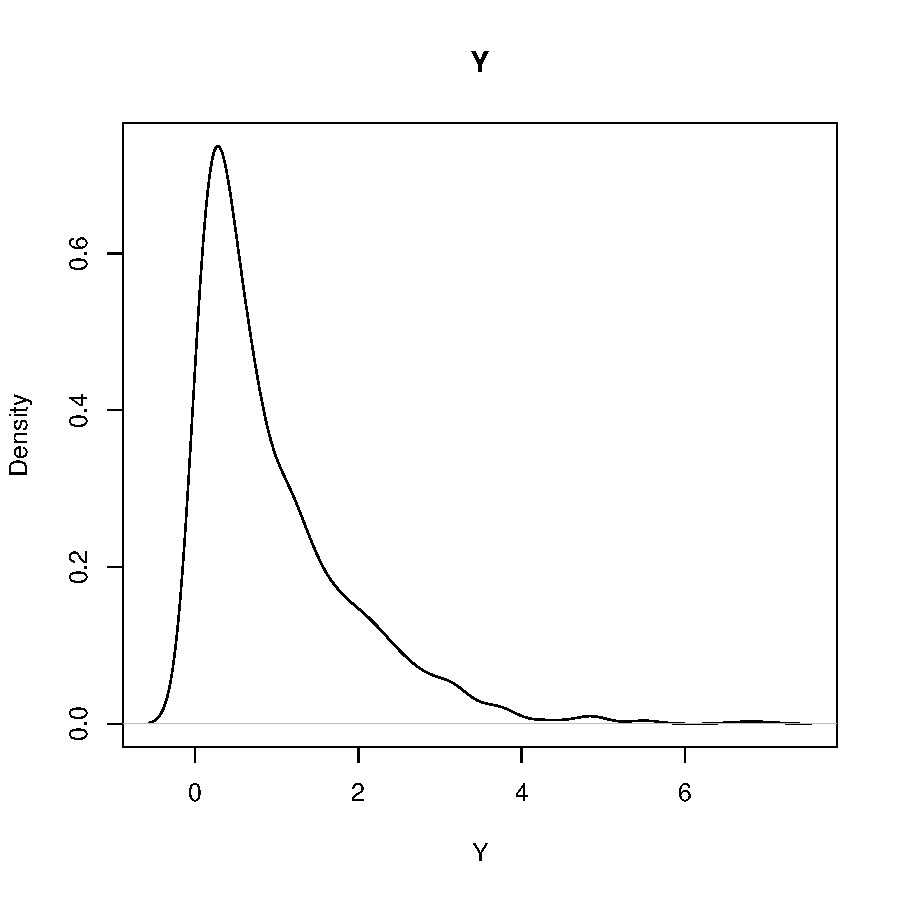
\includegraphics[width = 1.9in, height = 1.9in]{survival_present-expo.pdf}}
\subfigure{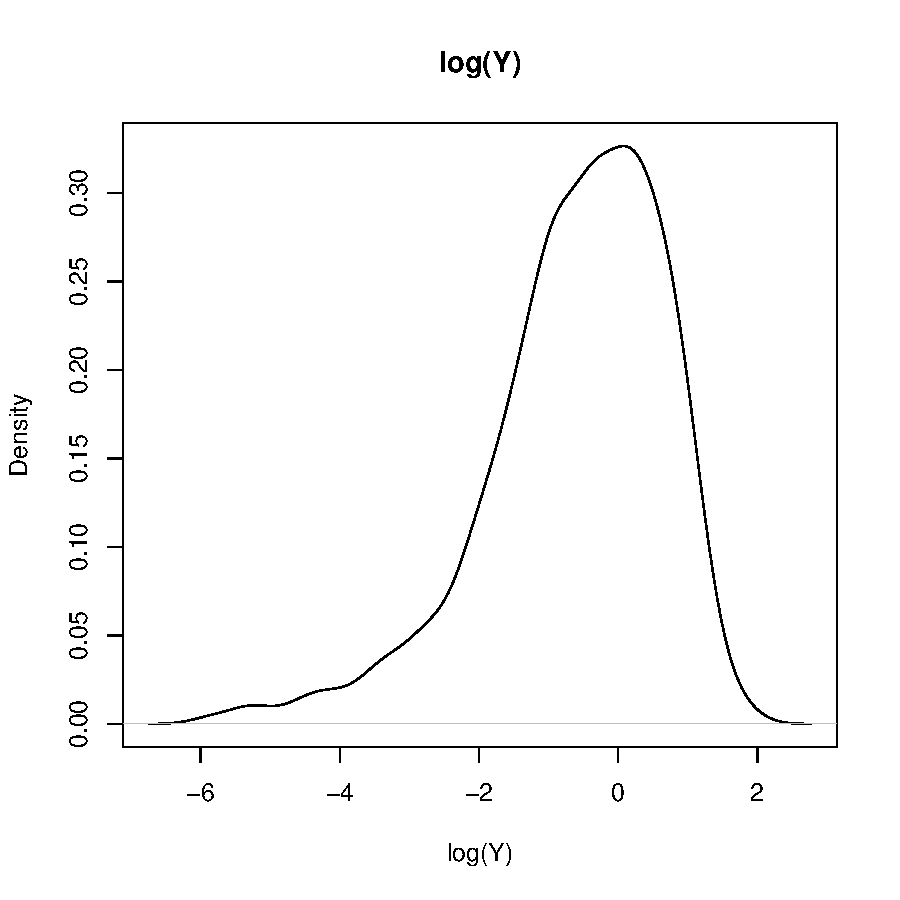
\includegraphics[width = 1.9in, height = 1.9in]{survival_present-logexpo.pdf}}
\end{center}
\end{figure}
\end{enumerate}
\end{frame}

\begin{frame}
\frametitle{Why not use OLS?}

\begin{enumerate}
\item[2.] Survival models can handle censoring.
\pause
\begin{center}
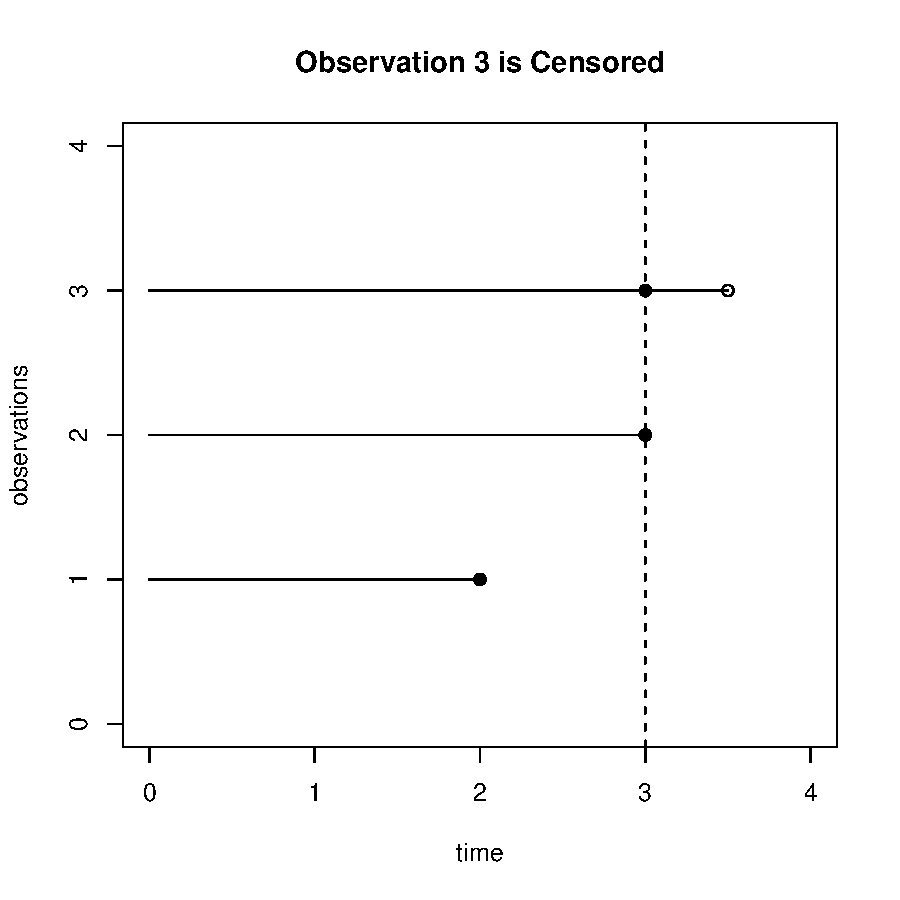
\includegraphics[width = 2in, height = 2in]{survival_present-censor.pdf}
\end{center}
\pause
Observation 3 is censored in that it has not experienced the event at
the time we stop collecting data, so we don't know its true duration.
\end{enumerate}
\end{frame}

\begin{frame}
\frametitle{Why not use OLS?}
\begin{enumerate}
\item[3.] Survival models can handle time-varying covariates (TVCs).
\begin{itemize}
\pause
\item If $Y$ is duration of a regime, GDP may change during the
duration of the regime.
\pause
\item OLS cannot handle multiple values of GDP per observation.
\pause
\item You can set up data in a special way with survival models such
that you can accomodate TVCs (not going to talk about this today).
\end{itemize}
\end{enumerate}
\end{frame}

\section{Underlying Math}

\begin{frame}
\frametitle{Outline}
\tableofcontents[currentsection]
\end{frame}

\begin{frame}
\frametitle{Probability Density Function}
\pause
Let $T$ be a continuous positive random variable denoting the duration/survival
times ($T = Y$).\\
\pause
\bigskip
$T$ has a \textbf{probability density function $f(t)$}: roughly
\emph{probability that an event occurs at time $t$}.
\pause
Because $f(t)$ is continuous, to get the probability, we would have to find the area
under the density for an infinitely small interval around $t$.
\pause
\begin{center}
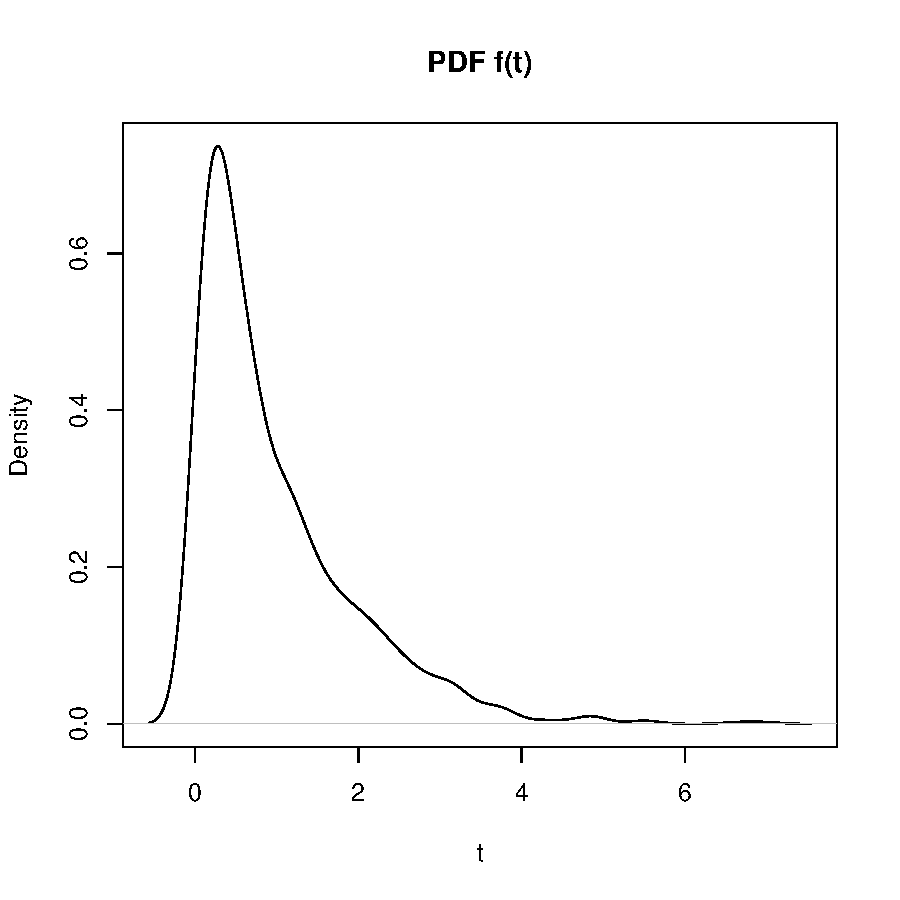
\includegraphics[width = 2in, height = 2in]{survival_present-pdf.pdf}
\end{center}
\end{frame}

\begin{frame}
\frametitle{Survivor Function}
\pause
$f(t)$ has a corresponding CDF $F(t) = \int_0^t f(u) du = P(T \le t)$,
which is the probability of an event occurring by time $t$.\\
\pause
\bigskip
Then the \textbf{survivor function} is $S(t) = 1 - F(t)$:
\emph{probability of surviving (no event) until at least time $t$}
\pause
\begin{figure}
\begin{center}
\subfigure{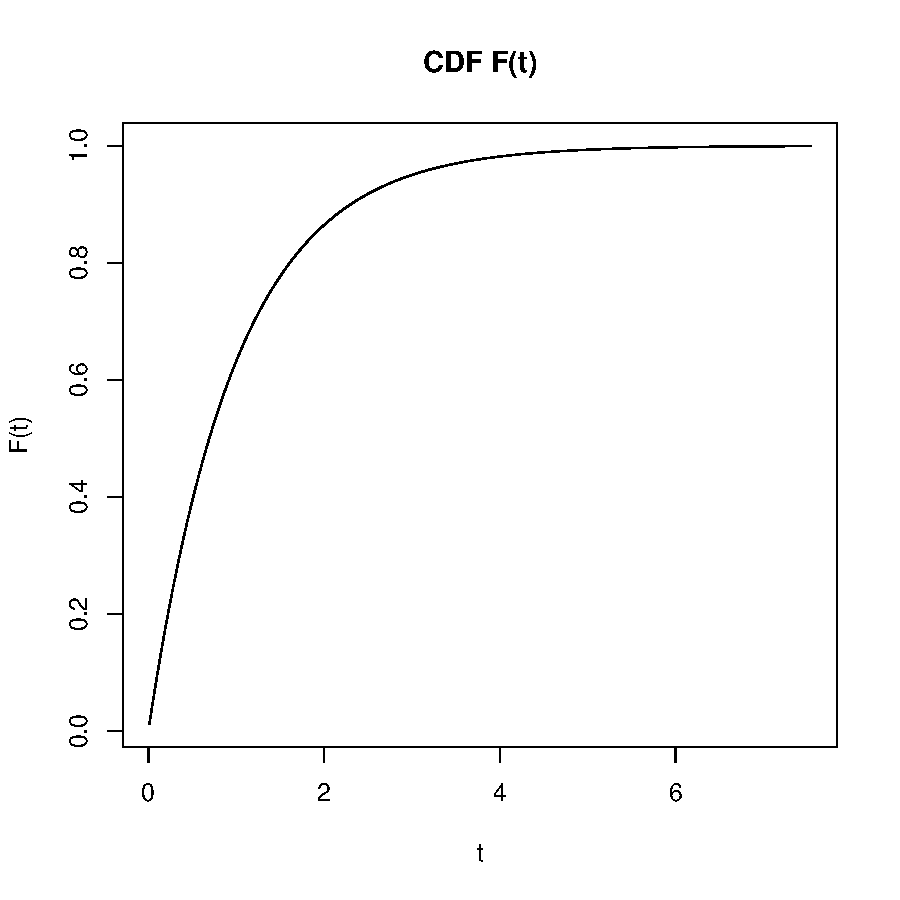
\includegraphics[width = 1.9in, height = 1.9in]{survival_present-cdf.pdf}}
\subfigure{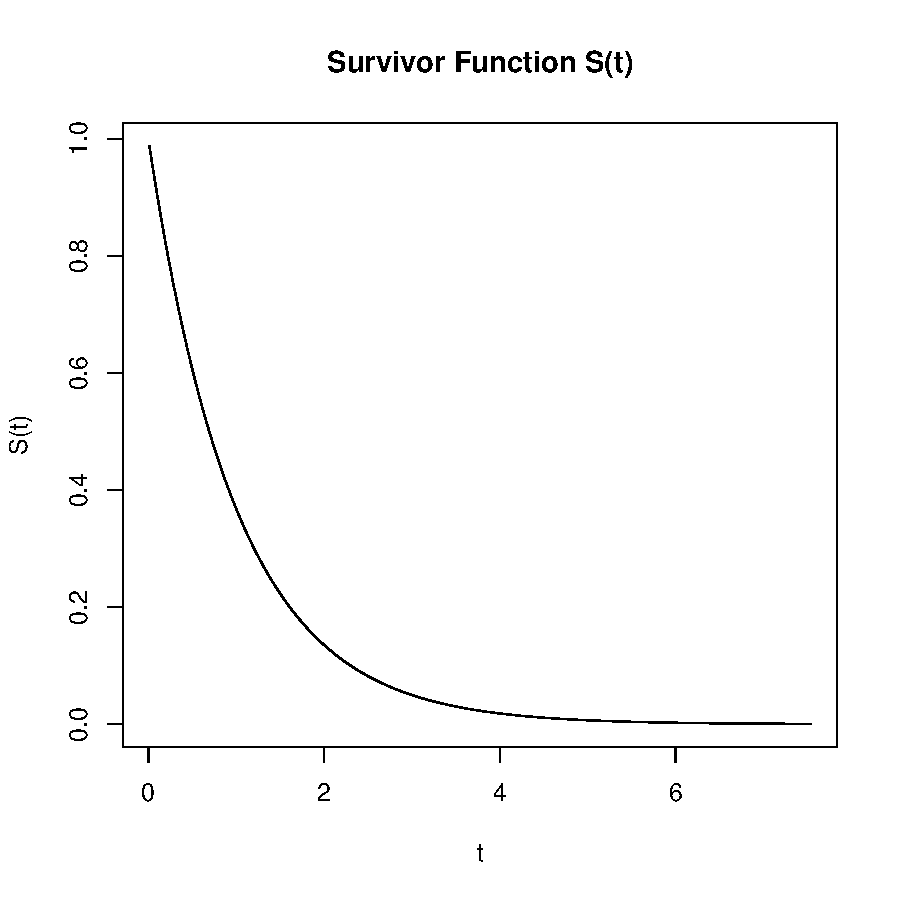
\includegraphics[width = 1.9in, height = 1.9in]{survival_present-survivor.pdf}}
\end{center}
\end{figure}
\end{frame}

\begin{frame}
\frametitle{Hazard Rate}
\pause
The \textbf{hazard rate} (or hazard function) $h(t)$ is roughly \emph{the
probability of an event at time $t$ given survival up to time $t$}.\\
\pause

\begin{eqnarray*}
h(t) &=& P(\mathrm{event \; at}\; t | \mathrm{survival \; up \; to} \; t)\\
\pause
&=& \frac{P(\mathrm{survival \; up \; to\; } t | \mathrm{event \; at}
\; t)P(\mathrm{event \; at} \; t)}{P(\mathrm{survival \; up \; to} \; t)}\\
\pause
&=& \frac{P(\mathrm{event \; at \; }t)}{P(\mathrm{survival \; up \;
to} \;  t)}\\
\pause
&=& \frac{f(t)}{S(t)}\\
\pause
f(t) &=& h(t) S(t) 
\end{eqnarray*}
\end{frame}

\begin{frame}
\begin{itemize}
\item The hazard rate has a substantive interpretation:
\pause
\begin{itemize}
\item Given a government has survived 2 years, what is the probability it will collapse?
\end{itemize}
\pause
\item Note that the hazard rate is a function of time:
\pause
\begin{itemize}
\item Increasing hazard: A government that has survived 2 years is
more likely to collapse than one that has survived 1 year.
\pause
\item Decreasing hazard: A government that has survived 2 years is
less likely to collapse than one that has survived 1 year.
\pause
\item Flat hazard: A government that has survived 2 years is no more
or less likely to collapse than one that has survived 1 year.
\end{itemize}
\pause
\item Parametric models usually assume some shape for the hazard
rate (i.e. flat, monotonic, etc.). 
\end{itemize}
\end{frame}

\begin{frame}
\frametitle{Modeling with Covariates}
\pause
We usually model the hazard rate as a function of covariates.
\pause
\begin{equation*}
h_i(t) = g(X_i \beta)
\end{equation*}
\pause
We can then interpret the change in the hazard rate and also the
change in average duration given a change in X (via the math from before).\\
\pause
\bigskip
When all the covariates are 0, $h_i(t) = g(\beta_0)$.  We call this the
\textbf{baseline hazard}. 
\end{frame}

\begin{frame}
\frametitle{Estimation of the Parameters}
Question: How do we estimate the parameters of interest?\\
\pause
\bigskip 
Answer: Use maximum likelihood estimation.
\end{frame}

\begin{frame}
\frametitle{A Brief Review (or Preview) of Maximum Likelihood}
\pause
We want to find a set of parameters $\theta$ (which include $\beta$
and possibly other ancillary parameters) given that we have data $y$.
\pause
\begin{eqnarray*}
P(\theta | y) &=& \frac{P(y|\theta)P(\theta)}{P(y)}\\
\pause
 &=& k(y) P(y|\theta)\\
\pause
&\propto& P(y|\theta)\\
\pause
\mathcal{L}(\theta | y) &=& \prod_{i=1}^n P(y_i|\theta) \; \mathrm{by \; i.i.d}
\pause
\end{eqnarray*}
The maximum point of $\mathcal{L}(\theta | y)$ in multi-dimensional space is the
MLE of our parameters.  \pause In our case,
\begin{equation*}
P(y|\theta) = f(t)
\end{equation*}
\end{frame}

\begin{frame}
\frametitle{What about Censoring?}
\pause
Observations that are censored give us no information about when the
event occurs, but they do give us information about how long they survive.\\
\pause
\bigskip
For censored observations, we know that they survived at least up to some
observed time $t^c$ and that their true duration is some $t^* \ge t^c$.\\
\pause
\bigskip
For each observation, create a censoring indicator $c_i$ such that 
\begin{eqnarray*}
c_i = \left \lbrace \begin{array}{l l}1 & \mathrm{if \; not \; censored}\\
0 & \mathrm{if \; censored}\end{array} \right.
\end{eqnarray*}
\end{frame}

\begin{frame}
We can incorporate the information from the censored observations into
the likelihood function.
\pause
\begin{eqnarray*}
\mathcal{L} &=& \prod^n_{i=1} \; \left[ f(t_i) \right] ^
{c_i} \; \left[ P(T_i^* \ge t_i^c) \right] ^ {1 - c_i}\\
\pause
&=& \prod^n_{i=1} \; \left[ f(t_i) \right] ^
{c_i} \; \left[ 1 - F(t_i) \right] ^ {1 - c_i} \\ 
\pause
&=& \prod^n_{i=1} \; \left[ f(t_i) \right] ^
{c_i} \; \left[ S(t_i) \right] ^ {1 - c_i} \\  
\end{eqnarray*}
\pause
So uncensored observations contribute to the density function and
censored observations contribute to the survivor function in the likelihood.
\end{frame}

\section{Parametric Survival Models}

\begin{frame}
\frametitle{Outline}
\tableofcontents[currentsection]
\end{frame}

\begin{frame}
\frametitle{Estimating Parametric Survival Models}
\pause
\begin{enumerate}
\item Make an assumption that $T_i$ follows a specific distribution
$f(t)$ (stochastic component).
\begin{itemize}
\pause
\item By making an assumption about $f(t)$, you are also making an
assumption about the shape of $h(t)$.
\end{itemize} 
\pause
\item Model the hazard rate with covariates (systematic component).
\pause
\item Estimate via ML.
\pause
\item Interpret quantities of interest (hazard ratios, expected
survival times).
\end{enumerate}
\end{frame}

\begin{frame}
\frametitle{Running Example: Duration of Parliamentary Cabinets}
\pause
\begin{itemize}
\item Example taken from King et al.\ (1990).
\pause
\item Dependent variable: number of months a coalition government
stays in power
\pause
\item Event: fall of a coalition government
\pause
\item Independent variables: 
\pause
\begin{itemize}
\item investiture ({\tt invest}): legal requirement for
legislature to approve cabinet
\pause
\item fractionalization ({\tt fract}): index characterizing the number
and size of parties in parliament, where higher numbers indicate
larger number of small blocs
\pause
\item polarization ({\tt polar}): measure of support for extremist parties
\pause
\item numerical status ({\tt numst2}): dummy variable coding majority
(1) or minority (0) government
\pause
\item crisis duration ({\tt crisis}): number of days of ``crisis''
before government is formed
\end{itemize}
\pause
\item Censoring occurs because of constitutionally mandated elections:
governments fall apart in anticipation of such elections
\end{itemize}
\end{frame}

\begin{frame}
\frametitle{The Exponential Model}
\pause
Assume:
\begin{eqnarray*}
T_i &\sim& \mathrm{Exponential}(\lambda_i)\\
\pause
E(T_i) &=& \frac{1}{\lambda_i}
\end{eqnarray*}
\pause
$\lambda_i > 0$ and is known as the rate parameter.
\begin{center}
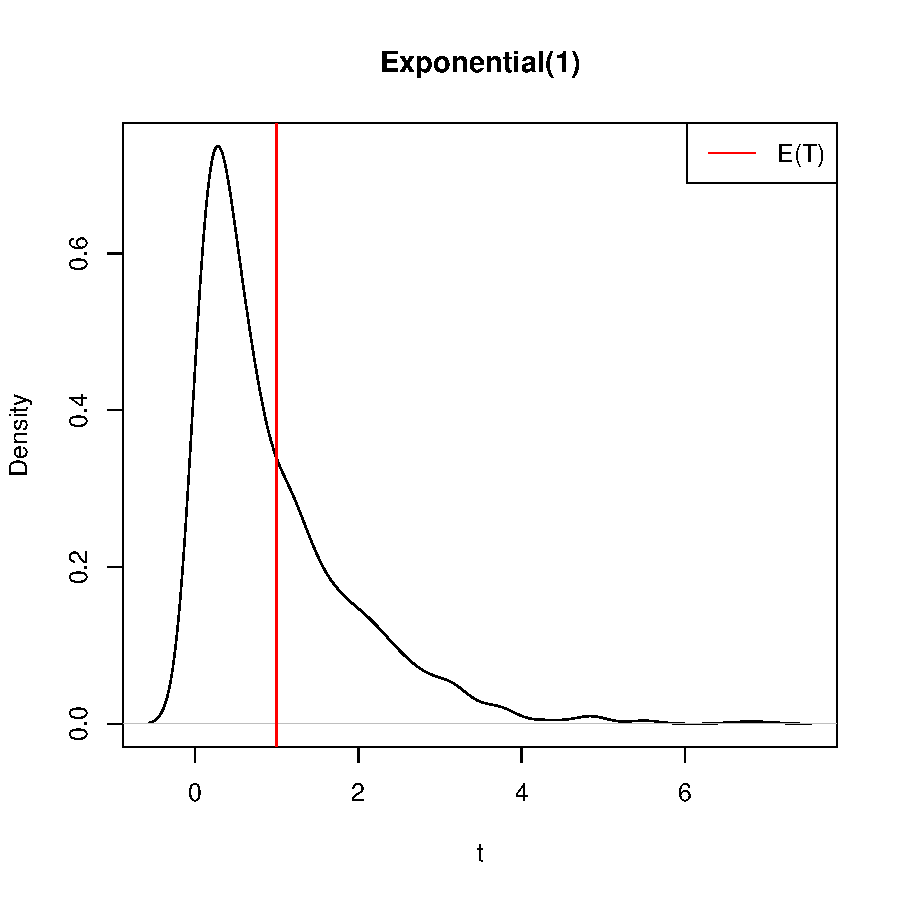
\includegraphics[width = 2in, height = 2in]{survival_present-expo1.pdf}
\end{center}

\end{frame}

\begin{frame}
\begin{eqnarray*}
f(t) &=& \lambda e^{-\lambda t}\\\\
\pause
S(t) &=& 1 - F(t)\\
\pause
&=& 1 - (1 - e^{-\lambda t})\\
\pause
&=& e^{-\lambda t}\\\\
\pause
h(t) &=& \frac{f(t)}{S(t)}\\
\pause
&=& \frac{\lambda e^{-\lambda t}}{e^{-\lambda t}}\\
\pause
&=& \lambda
\end{eqnarray*}
\end{frame}

\begin{frame}
Modeling $h(t)$ with covariates:
\pause
\begin{eqnarray*}
h(t_i) &=& \lambda_i\\
\end{eqnarray*}
\pause
We want to constrain the $h(t)$ to be positive.
\pause
\begin{eqnarray*}
\lambda_i &=& e^{-\mathbf{x}_i \beta}
\end{eqnarray*}
\pause
Positive $\beta$ implies that hazard decreases and average survival
time increases as $x$ increases.\\
\bigskip
\pause
Because $h(t_i)$ is modeled with only one parameter $\lambda_i$ and is
not a function of $t_i$, the
exponential model assumes a \textbf{flat hazard} (no time dependence). \pause This
corresponds to the memoryless property of the exponential distribution.
\end{frame}

\begin{frame}
Estimation via ML:
\pause
\begin{eqnarray*}
\mathcal{L} &=& \prod^n_{i=1} \; \left[ f(t_i) \right] ^
{c_i} \; \left[ S(t_i) \right] ^ {1 - c_i} \\  
\pause 
&=&  \prod^n_{i=1} \; \left[ \lambda_i e^{-\lambda_i t_i} \right] ^{c_i}
\; \left[ e^{-\lambda_i t_i} \right] ^ {1 - c_i}\\
\pause
\mathrm{ln} \; \mathcal{L} &=& \sum_{i=1}^n \; c_i \; (\mathrm{ln} \;
\lambda_i - \lambda_i t_i) + (1-c_i) (-\lambda_i t_i) \\
\pause
&=& \sum_{i=1}^n \; c_i \; (\mathrm{ln} \;
e^{-\mathbf{x}_i \beta} - e^{-\mathbf{x}_i \beta} t_i) + (1-c_i) (-e^{-\mathbf{x}_i \beta} t_i) \\
\pause
&=& \sum_{i=1}^n \; c_i \; (\mathrm{ln} \;
e^{-\mathbf{x}_i \beta} - e^{-\mathbf{x}_i \beta} t_i +
e^{-\mathbf{x}_i \beta} t_i) - e^{-\mathbf{x}_i \beta} t_i\\
\pause
&=& \sum_{i=1}^n \; c_i \; (-\mathbf{x}_i \beta) - e^{-\mathbf{x}_i \beta} t_i\\
\end{eqnarray*}
\end{frame}

\begin{frame}[fragile]
\begin{equation*}
\mathrm{ln} \; \mathcal{L} = \sum_{i=1}^n \; c_i \; (-\mathbf{x}_i \beta) - e^{-\mathbf{x}_i \beta} t_i
\end{equation*}
\pause
\tiny{
\begin{Schunk}
\begin{Sinput}
> data(coalition)
\end{Sinput}
\end{Schunk}
\begin{Schunk}
\begin{Sinput}
> X <- as.matrix(cbind(1, coalition[, c("invest", "fract", "polar", 
+     "numst2", "crisis")]))
> T <- coalition$duration
> C <- coalition$ciep12
\end{Sinput}
\end{Schunk}
\pause
\begin{Schunk}
\begin{Sinput}
> expo.lik <- function(par, T, X, C) {
+     beta <- par
+     lambda <- exp(-(X %*% beta))
+     log.lik <- sum(C * (-(X %*% beta)) - (lambda * T))
+     return(log.lik)
+ }
\end{Sinput}
\end{Schunk}
\pause
\begin{Schunk}
\begin{Sinput}
> my.coef <- optim(par = c(0, 0, 0, 0, 0, 0), fn = expo.lik, T = T, 
+     X = X, C = C, method = "BFGS", control = list(fnscale = -1))$par
\end{Sinput}
\end{Schunk}
}
\end{frame}

\begin{frame}[fragile]
Or we can use the {\tt survival} (or {\tt Zelig}) package in R:
\pause
\bigskip
\tiny{
\begin{Schunk}
\begin{Sinput}
> library(survival)
\end{Sinput}
\end{Schunk}
\pause
\begin{Schunk}
\begin{Sinput}
> expo.surv <- survreg(Surv(duration, ciep12) ~ invest + fract + 
+     polar + numst2 + crisis, data = coalition, dist = "exponential")
\end{Sinput}
\end{Schunk}
\pause
\begin{Schunk}
\begin{Sinput}
> expo.surv$coef
\end{Sinput}
\begin{Soutput}
(Intercept)      invest       fract       polar      numst2      crisis 
   4.826723   -0.504758   -2.250355   -0.028796    0.461321    0.005587 
\end{Soutput}
\begin{Sinput}
> my.coef
\end{Sinput}
\begin{Soutput}
[1]  4.828623 -0.504985 -2.253515 -0.028797  0.461015  0.005603
\end{Soutput}
\end{Schunk}
\pause
\begin{Schunk}
\begin{Sinput}
> expo.surv$loglik[2]
\end{Sinput}
\begin{Soutput}
[1] -1046
\end{Soutput}
\begin{Sinput}
> expo.lik(par = my.coef, X = X, T = T, C = C)
\end{Sinput}
\begin{Soutput}
[1] -1046
\end{Soutput}
\end{Schunk}
}
\end{frame}

\begin{frame}[fragile]
How do we get quantities of interest?\\
\pause
\bigskip
Variable of interest: majority versus minority governments ({\tt
numst2}), with all other variables set at mean or mode.\\
\pause
\tiny{
\bigskip
\begin{Schunk}
\begin{Sinput}
> x.min <- colMeans(model.matrix(expo.surv))
> x.min[c("invest", "numst2")] <- 0
> x.maj <- x.min
> x.maj["numst2"] <- 1
\end{Sinput}
\end{Schunk}
\pause
\begin{Schunk}
\begin{Sinput}
> x.min
\end{Sinput}
\begin{Soutput}
(Intercept)      invest       fract       polar      numst2      crisis 
     1.0000      0.0000      0.7188     15.2898      0.0000     22.3822 
\end{Soutput}
\begin{Sinput}
> x.maj
\end{Sinput}
\begin{Soutput}
(Intercept)      invest       fract       polar      numst2      crisis 
     1.0000      0.0000      0.7188     15.2898      1.0000     22.3822 
\end{Soutput}
\end{Schunk}
\bigskip
\normalsize
Simulating Estimation Uncertainty:
\pause
\tiny{
\begin{Schunk}
\begin{Sinput}
> betas <- mvrnorm(1000, mu = expo.surv$coef, Sigma = vcov(expo.surv))
\end{Sinput}
\end{Schunk}
}
}
\end{frame}

\begin{frame}[fragile]

\pause
\bigskip
\normalsize
Hazard Ratios:
\begin{eqnarray*}
\mathrm{HR} &=& \frac{h(t | \mathbf{x}_{\mathrm{maj}})}{h(t | \mathbf{x}_{\mathrm{min}})}\\
\pause
&=& \frac{e^{-\mathbf{x}_{\mathrm{maj}}\beta }}{e^{-\mathbf{x}_{\mathrm{min}}\beta }}\\
\pause
&=& \frac{e^{-\beta_0}e^{-x_1 \beta_1}e^{-x_2 \beta_2} e^{-x_3
\beta_3} e^{-x_{\mathrm{maj}} \beta_4} e^{-x_5 \beta_5}}{e^{-\beta_0}e^{-x_1 \beta_1}e^{-x_2 \beta_2} e^{-x_3
\beta_3} e^{-x_{\mathrm{min}} \beta_4} e^{-x_5 \beta_5}}\\
\pause
&=& \frac{e^{-x_{\mathrm{maj}} \beta_4}}{e^{-x_{\mathrm{min}} \beta_4}}\\
\pause
&=& e^{-\beta_4}
\end{eqnarray*}
\pause
Hazard ratio greater than 1 implies that majority governments fall
faster (shorter survival time) than minority governments.  \\
\pause 
\bigskip
Constant hazard ratio across time is the \emph{proportional hazards assumption}.
\end{frame}

\begin{frame}[fragile]
\tiny
\begin{Schunk}
\begin{Sinput}
> hr.1 <- exp(-betas[, "numst2"])
\end{Sinput}
\end{Schunk}
\pause
\begin{Schunk}
\begin{Sinput}
> hr.2 <- exp(-x.maj %*% t(betas))/exp(-x.min %*% t(betas))
\end{Sinput}
\end{Schunk}
\pause
\begin{Schunk}
\begin{Sinput}
> all.equal(hr.1, as.numeric(hr.2))
\end{Sinput}
\begin{Soutput}
[1] TRUE
\end{Soutput}
\end{Schunk}
\pause

\begin{center}
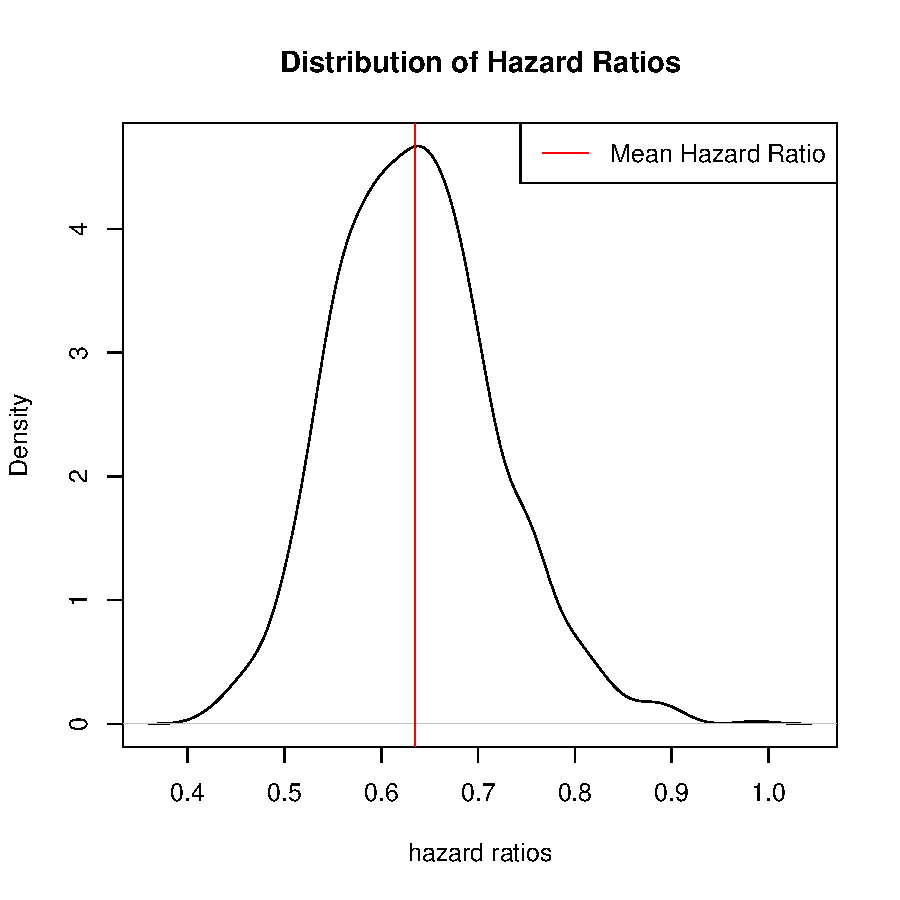
\includegraphics[width = 2in, height = 2in]{survival_present-hr.pdf}
\end{center}
\normalsize
\pause
Majority governments survive longer than minority governments.
\end{frame}

\begin{frame}[fragile]
Expected (average) Survival Time:
\pause
\begin{eqnarray*}
E(T | \mathbf{x}_i) &=& \frac{1}{\lambda_i}\\
\pause
&=& \frac{1}{e^{-\mathbf{x}_i \beta}}
\end{eqnarray*}
\pause
\tiny
\begin{Schunk}
\begin{Sinput}
> expect.maj <- 1/exp(-x.maj %*% t(betas))
> expect.min <- 1/exp(-x.min %*% t(betas))
\end{Sinput}
\end{Schunk}
\pause
\begin{center}
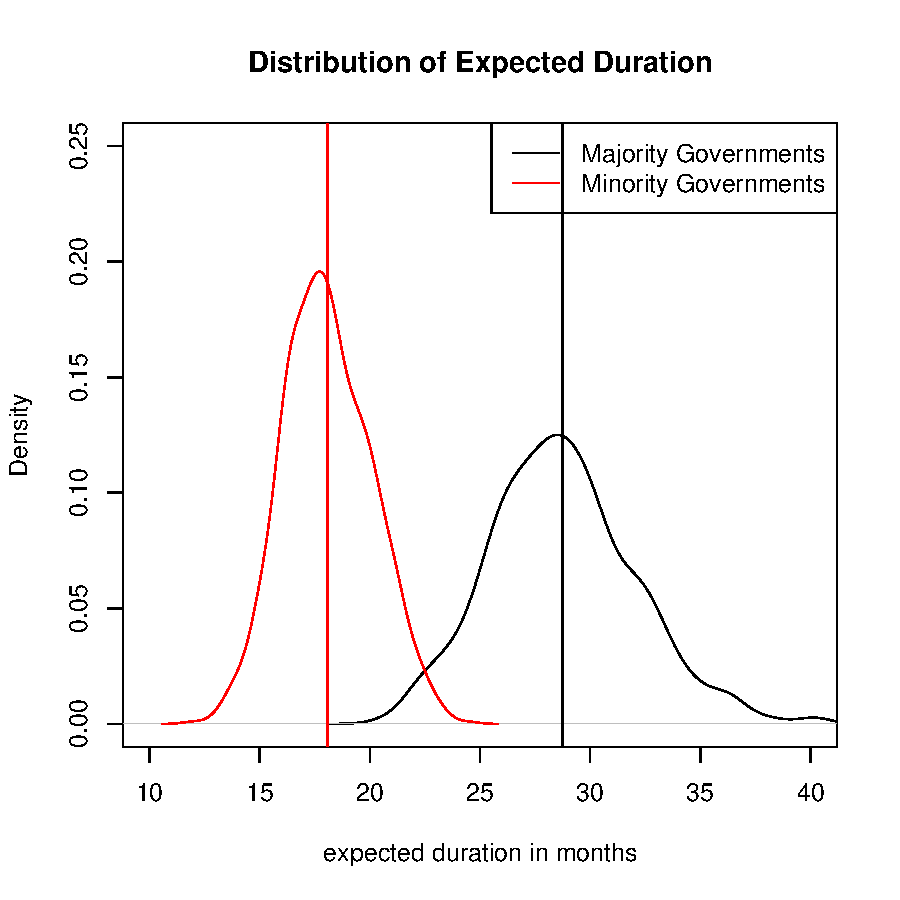
\includegraphics[width = 2in, height = 2in]{survival_present-expected.pdf}
\end{center}

\end{frame}

\begin{frame}[fragile]
\normalsize
Predicted Survival Time:\\
\pause
\bigskip
Draw predicted values from the exponential distribution.
\pause
\tiny
\begin{Schunk}
\begin{Sinput}
> predict.maj <- apply(X = 1/expect.maj, MARGIN = 2, FUN = rexp, 
+     n = 1)
> predict.min <- apply(X = 1/expect.min, MARGIN = 2, FUN = rexp, 
+     n = 1)
\end{Sinput}
\end{Schunk}
\pause
\begin{center}
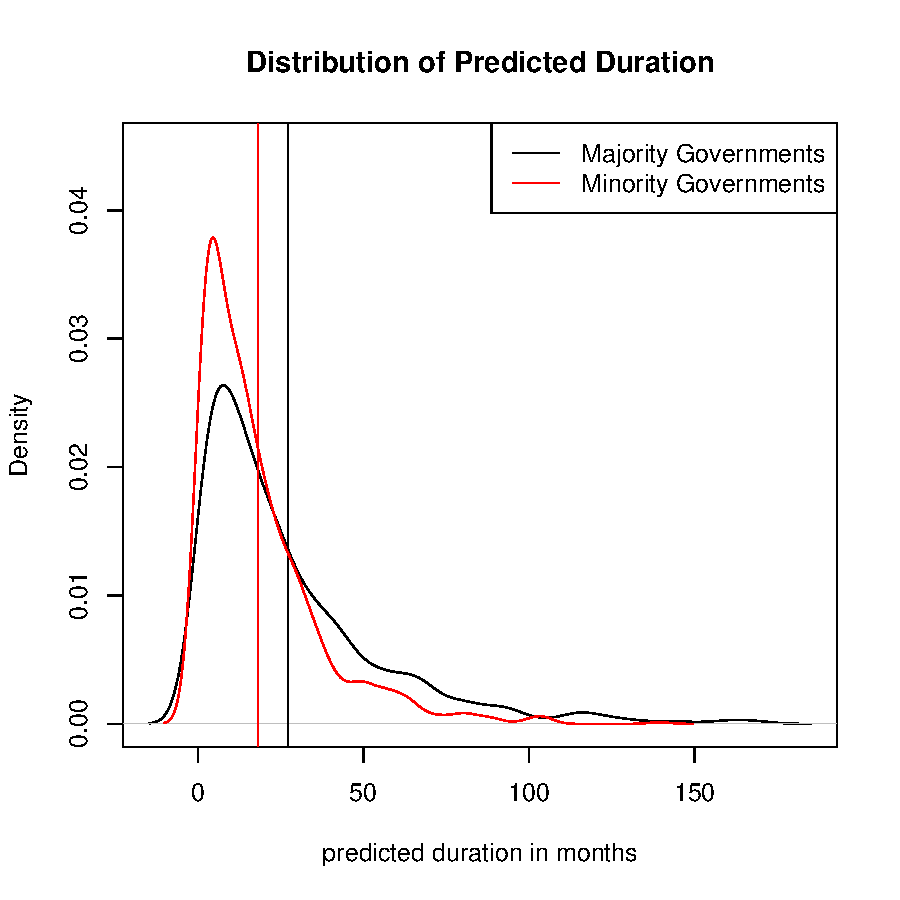
\includegraphics[width = 2in, height = 2in]{survival_present-predicted.pdf}
\end{center}

\end{frame}

\begin{frame}[fragile]
\normalsize
First Differences:
\pause
\begin{eqnarray*}
E(T | \mathbf{x}_\mathrm{maj}) - E(T | \mathbf{x}_\mathrm{min})
\end{eqnarray*}
\pause
\tiny
\begin{Schunk}
\begin{Sinput}
> first.diff <- expect.maj - expect.min
\end{Sinput}
\end{Schunk}
\pause
\begin{center}
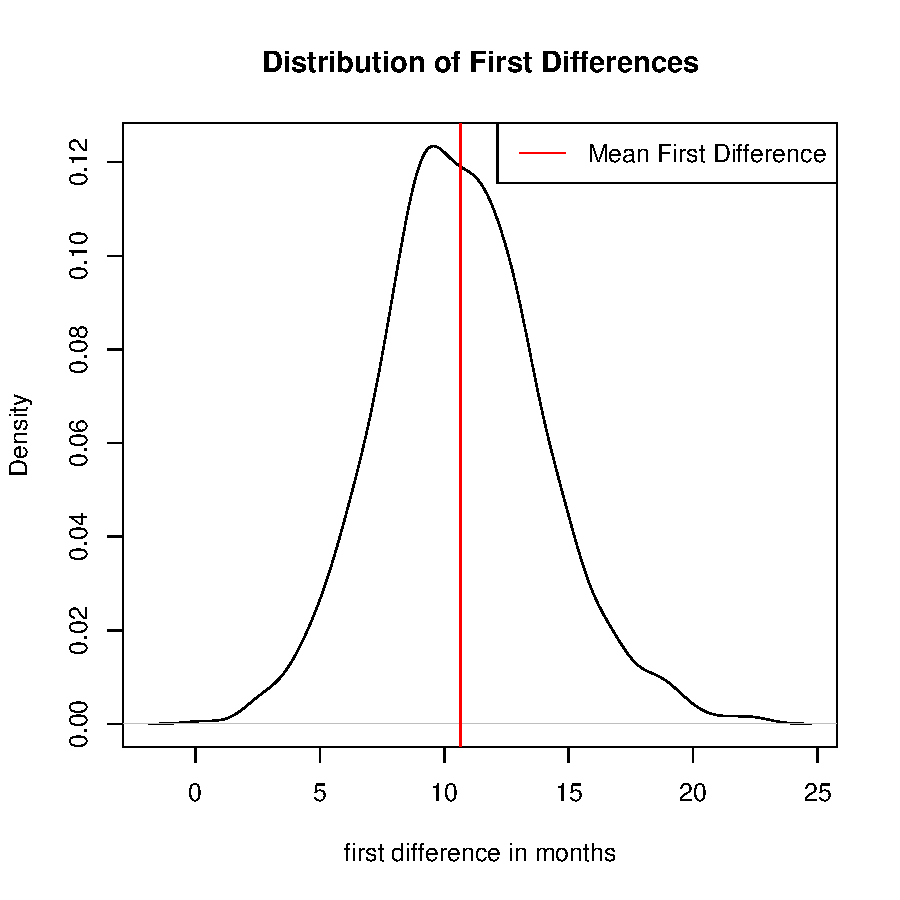
\includegraphics[width = 2in, height = 2in]{survival_present-fd.pdf}
\end{center}

\end{frame}

\begin{frame}
\normalsize
The exponential model is nice and simple, but the assumption of a flat
hazard may be too restrictive.\\
\pause
\bigskip
What if we want to loosen that restriction by assuming a monotonic hazard?\\
\pause
\bigskip
We can use the Weibull model.
\end{frame}

\begin{frame}
\frametitle{The Weibull Model}
Assume:
\begin{eqnarray*}
T_i &\sim& \mathrm{Weibull}(\lambda_i, p)\\
\pause
E(T_i) &=& \lambda_i \Gamma \left( 1 + \frac{1}{p} \right)
\end{eqnarray*}
\pause
$\lambda_i > 0$ is known as the scale parameter and $p > 0$ is the shape parameter.
\pause
\begin{figure}
\begin{center}
\subfigure{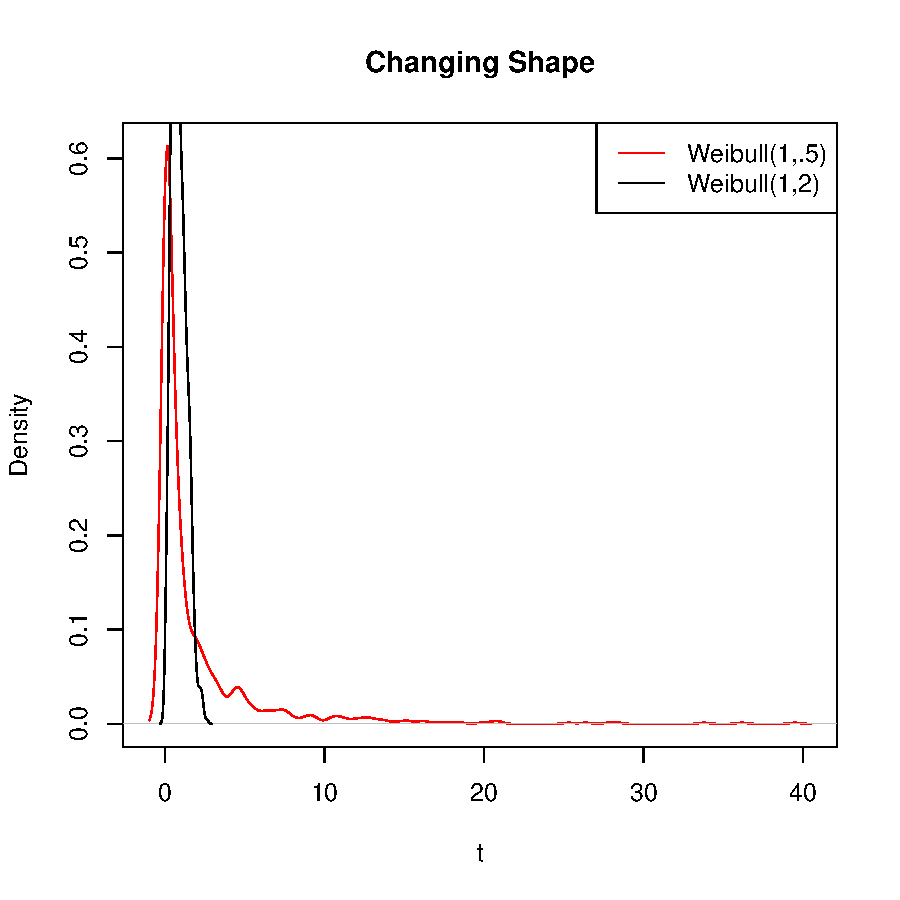
\includegraphics[width = 1.9in, height = 1.9in]{survival_present-weibull.pdf}}
\subfigure{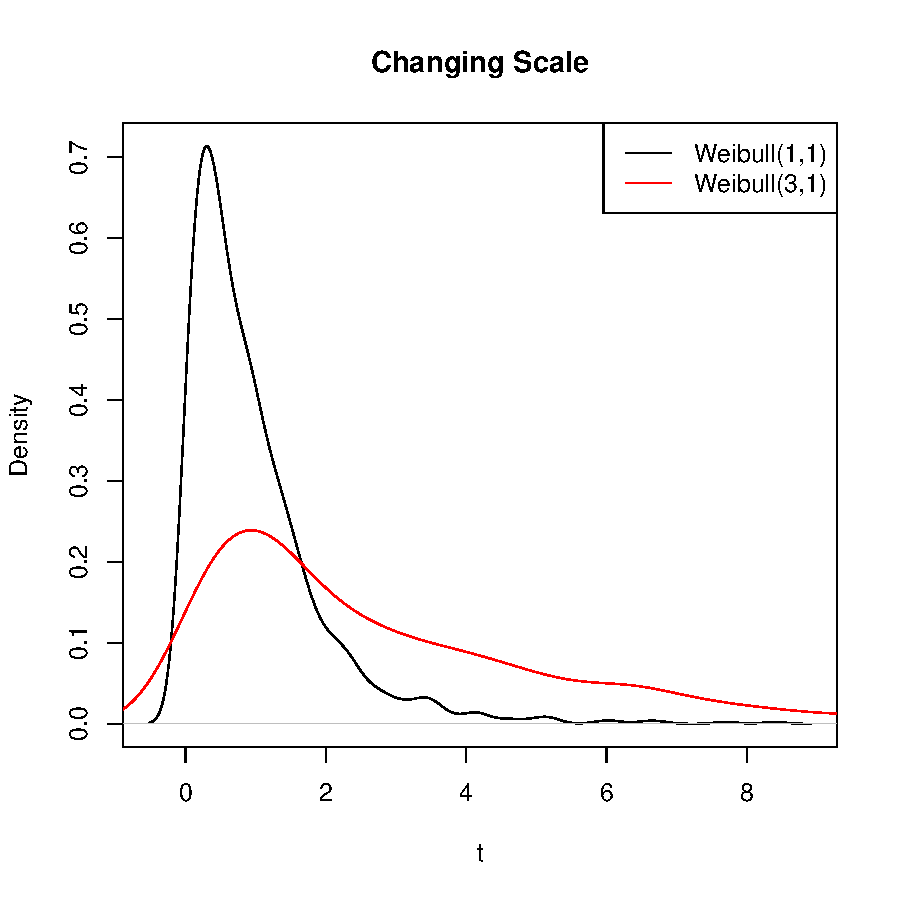
\includegraphics[width = 1.9in, height = 1.9in]{survival_present-weibull2.pdf}}
\end{center}
\end{figure}
\end{frame}

\begin{frame}
\begin{eqnarray*}
f(t) &=& \left( \frac{p}{\lambda} \right) \left( \frac{t}{\lambda}
\right) ^ {p-1} e^{-(t/\lambda)^p} \\\\
\pause
S(t) &=& 1 - F(t) \\
\pause
&=& 1 - (1 - e^{-(t/\lambda)^p})\\
\pause
&=& e^{-(t/\lambda)^p}\\\\
\pause
h(t) &=& \frac{f(t)}{S(t)}\\
\pause
&=& \dfrac{\left( \frac{p}{\lambda} \right) \left( \frac{t}{\lambda}
\right) ^ {p-1} e^{-(t/\lambda)^p}}{e^{-(t/\lambda)^p}}\\
\pause
&=& \left( \frac{p}{\lambda} \right) \left( \frac{t}{\lambda}
\right) ^ {p-1}\\
\pause
&=& \left( \frac{p}{\lambda ^p} \right) t^{p-1}
\end{eqnarray*}
\end{frame}

\begin{frame}
Modeling $h(t)$ with covariates:
\pause
\begin{eqnarray*}
h(t_i) &=& \left( \frac{p}{\lambda_i ^p} \right) t_i^{p-1}\\
\end{eqnarray*}
\pause
We want to constrain the $h(t)$ to be positive.
\pause
\begin{eqnarray*}
\lambda_i &=& e^{\mathbf{x}_i \beta}
\end{eqnarray*}
\pause
Note that the link is different from the exponential model.  \pause Positive
$\beta$ implies that hazard decreases and average survival time increases as $x$ increases.\\
\end{frame}

\begin{frame}
$h(t_i)$ is modeled with both $\lambda_i$ and $p$ and is a function of
$t_i$. Thus, the
Weibull model assumes a \textbf{monotonic hazard}.
\pause
\begin{itemize}
\item If $p = 1$, $h(t)$ is flat and the model is the exponential
model.
\pause
\item If $p > 1$, $h(t)$ is monotonically increasing.
\pause
\item If $p < 1$, $h(t)$ is monotonically decreasing.
\end{itemize}
\pause
\begin{center}
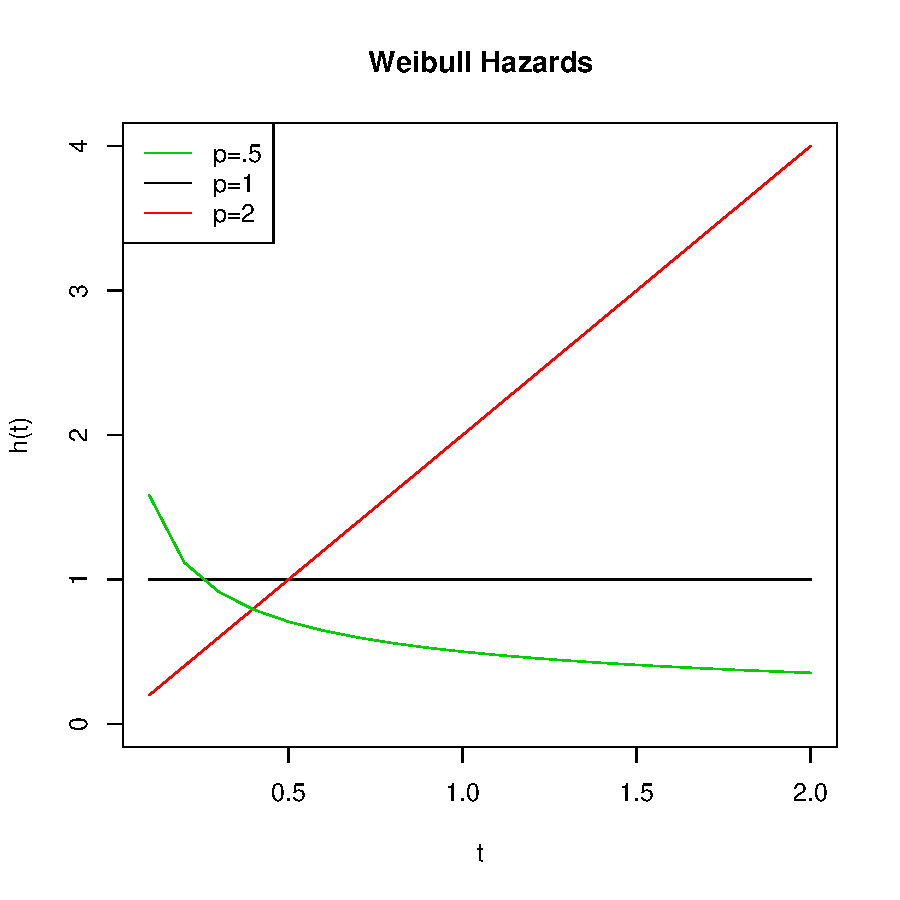
\includegraphics[width = 2in, height = 2in]{survival_present-weibhaz.pdf}
\end{center}
\end{frame}

\begin{frame}
\begin{eqnarray*}
\mathcal{L} &=& \prod^n_{i=1} \; \left[ f(t_i) \right] ^
{c_i} \; \left[ S(t_i) \right] ^ {1 - c_i} \\  
\pause 
&=&  \prod^n_{i=1} \; \left[  \left( \frac{p}{\lambda} \right) \left( \frac{t}{\lambda}
\right) ^ {p-1} e^{-(t/\lambda)^p} \right] ^
{c_i} \; \left[ e^{-(t/\lambda)^p} \right] ^ {1 - c_i} \\  
\pause
&=&  \prod^n_{i=1} \; \left[  \left( \frac{p}{\lambda ^p} \right) t^{p-1} e^{-(t/\lambda)^p} \right] ^{c_i} \; \left[ e^{-(t/\lambda)^p} \right] ^ {1 - c_i} \\  
\pause
\mathrm{ln} \; \mathcal{L} &=& \sum_{i=1}^n c_i \left[ \mathrm{ln} \;
p - p \; \mathrm{ln} \; \lambda + (p-1) \; \mathrm{ln} \; t_i \right] - \left(
\frac{t_i}{\lambda} \right) ^p\\
\pause
&=& \sum_{i=1}^n c_i \left[ \mathrm{ln} \;
p - p \; \mathbf{x}_i \beta + (p-1) \; \mathrm{ln} \; t_i \right] - \left(
\frac{t_i}{ e^{\mathbf{x}_i \beta}} \right) ^p\\
\end{eqnarray*}
\end{frame}

\begin{frame}[fragile]
Maximizing your own likelihood:
\pause
\tiny
\begin{Schunk}
\begin{Sinput}
> weib.lik <- function(par, T, X, C) {
+     beta <- par[1:ncol(X)]
+     p <- exp(par[(ncol(X) + 1)])
+     lambda <- exp((X %*% beta))
+     log.lik <- sum(C * (log(p) - p * log(lambda) + (p - 1) * 
+         log(T)) - (T/lambda)^p)
+     return(log.lik)
+ }
\end{Sinput}
\end{Schunk}
\pause
\begin{Schunk}
\begin{Sinput}
> my.max <- optim(par = c(0, 0, 0, 0, 0, 0, 0), fn = weib.lik, 
+     T = T, X = X, C = C, method = "BFGS", control = list(fnscale = -1))$par
> my.coef <- my.max[1:ncol(X)]
> my.p <- exp(my.max[(ncol(X) + 1)])
\end{Sinput}
\end{Schunk}
\pause
\normalsize
\bigskip
Using the {\tt survival} package:
\tiny
\begin{Schunk}
\begin{Sinput}
> weib.surv <- survreg(Surv(duration, ciep12) ~ invest + fract + 
+     polar + numst2 + crisis, data = coalition, dist = "weibull")
\end{Sinput}
\end{Schunk}
\end{frame}

\begin{frame}[fragile]
\tiny
\begin{Schunk}
\begin{Sinput}
> summary(weib.surv)
\end{Sinput}
\begin{Soutput}
Call:
survreg(formula = Surv(duration, ciep12) ~ invest + fract + polar + 
    numst2 + crisis, data = coalition, dist = "weibull")
               Value Std. Error     z        p
(Intercept)  4.75007    0.53072  8.95 3.55e-19
invest      -0.47160    0.11643 -4.05 5.11e-05
fract       -2.11762    0.75876 -2.79 5.26e-03
polar       -0.02792    0.00506 -5.52 3.33e-08
numst2       0.42746    0.11025  3.88 1.06e-04
crisis       0.00538    0.00183  2.94 3.28e-03
Log(scale)  -0.15644    0.04971 -3.15 1.65e-03

Scale= 0.855 

Weibull distribution
Loglik(model)= -1042   Loglik(intercept only)= -1101
	Chisq= 117.8 on 5 degrees of freedom, p= 0 
Number of Newton-Raphson Iterations: 5 
n= 314 
\end{Soutput}
\end{Schunk}
\end{frame}

\begin{frame}[fragile]
\normalsize
The shape parameter $p$ for the Weibull distribution is the inverse of
the scale parameter given by {\tt survreg()}.  
\pause
\tiny
\begin{Schunk}
\begin{Sinput}
> surv.p <- 1/weib.surv$scale
\end{Sinput}
\end{Schunk}
\pause
\begin{Schunk}
\begin{Sinput}
> surv.p
\end{Sinput}
\begin{Soutput}
[1] 1.169
\end{Soutput}
\begin{Sinput}
> my.p
\end{Sinput}
\begin{Soutput}
[1] 1.169
\end{Soutput}
\end{Schunk}
\normalsize
\pause
\bigskip
The scale parameter given by {\tt survreg()} is NOT the same as the scale
parameter in the Weibull distribution, which should be $\lambda_i =
e^{\mathbf{x}_i \beta}$.
\bigskip
\pause 
\tiny
\begin{Schunk}
\begin{Sinput}
> rbind(weib.surv.coef = weib.surv$coef, my.coef)
\end{Sinput}
\begin{Soutput}
               (Intercept)  invest  fract    polar numst2   crisis
weib.surv.coef       4.750 -0.4716 -2.118 -0.02792 0.4275 0.005377
my.coef              4.753 -0.4719 -2.122 -0.02792 0.4271 0.005405
\end{Soutput}
\end{Schunk}
\end{frame}

\begin{frame}
\normalsize
\frametitle{Other Parametric Models}
\pause
\begin{itemize}
\item Gompertz or gamma model: monotonic hazard
\pause
\item Log-logistic or log-normal model: nonmonotonic hazard
\pause
\item Generalized gamma model: nests the exponential, Weibull,
log-normal, and gamma models with an extra parameter
\end{itemize}
\pause
\bigskip
But what if we don't want to make an assumption about the shape of the
hazard?
\end{frame}

\section{The Cox Proportional Hazards Model}

\begin{frame}
\frametitle{Outline}
\tableofcontents[currentsection]
\end{frame}

\begin{frame}
\frametitle{The Cox Proportional Hazards Model}
\pause
\begin{itemize}
\item Often described as a semi-parametric model.
\pause
\item Makes no assumptions about the shape of the hazard or the
distribution of $T_i$.
\pause
\item Takes advantage of the proportional hazards assumption.
\end{itemize}
\end{frame}

\begin{frame}
\begin{enumerate}
\item Reconceptualize each $t_i$ as a discrete event time rather than
a duration or survival time (non-censored observations only). 
\pause
\begin{itemize}
\item $t_i = 5$: An event occurred at month 5, rather than observation
$i$ surviving for 5 months.
\end{itemize}
\pause
\item Assume there are no tied event times in the data.
\pause
\begin{itemize}
\pause
\item No two events can occur at the same instant.  It only seems that
way because our unit of measurement is not precise enough.
\pause
\item There are ways to adjust the likelihood to take into account
observed ties.
\end{itemize}
\pause
\item Assume no events can happen between event times.
\end{enumerate}
\end{frame}

\begin{frame}
We know that exactly one event occurred at each $t_i$ for all
non-censored $i$. \\
\pause
\bigskip
Define a risk set $R_i$ as the set of all possible observations at
risk of an event at time $t_i$.\\
\pause
\bigskip
What observations belong in $R_i$?\\
\pause
\bigskip
All observations (censored and non-censored) $j$ such
that $t_j \ge t_i$\\
\pause
\bigskip
For example, if $t_i = 5$ months, then all observations that do not
experience the event or are not censored before 5 months are at risk.

\end{frame}

\begin{frame}
We can then create a \emph{partial likelihood} function:
\pause
\begin{eqnarray*}
\mathcal{L} &=& \prod_{i=1}^n \left[ P(\mathrm{event \; occurred \; in} \; i |
\mathrm{event \; occurred \; in} \; R_i) \right] ^{c_i}  \\
\pause
&=& \prod_{i=1}^n \left[ \frac{P(\mathrm{event \; occurred \; in} \;
i)}{P(\mathrm{event \; occurred \; in} \; R_i)} \right] ^{c_i} \\
\pause
&=& \prod_{i=1}^n \left[ \frac{h(t_i)}{\sum_{j \in R_i} h(t_j)}
\right] ^{c_i}\\
\pause
&=& \prod_{i=1}^n \left[ \frac{h_0(t)h_i(t_i)}{\sum_{j \in R_i} h_0(t)h_j(t_j)}
\right] ^{c_i}\\
\pause
&=& \prod_{i=1}^n \left[ \frac{h_i(t_i)}{\sum_{j \in R_i} h_j(t_j)}
\right] ^{c_i}\\
\end{eqnarray*}
\pause
$h_0(t)$ is the baseline hazard, which is the same for all
observations, so it cancels out.

\end{frame}

\begin{frame}
Like in parametric models, $h(t)$ is modeled with covariates:
\pause
\begin{eqnarray*}
h_i(t_i) = e^{\mathbf{x}_i \beta}
\end{eqnarray*}
\pause
Note that a positive $\beta$ now suggests that an increase in $x$
increases the hazard and decreases survival time.
\pause
\begin{eqnarray*}
\mathcal{L} &=& \prod_{i=1}^n \left[ \frac{e^{\mathbf{x}_i
\beta}}{\sum_{j \in R_i} e^{\mathbf{x}_j \beta}}
\right] ^{c_i} \\
\end{eqnarray*}
\pause
There is no $\beta_0$ term estimated.  
\pause
This implies that the shape of the baseline hazard is left unmodeled.
\end{frame}

\begin{frame}
Pros:
\pause
\begin{itemize}
\item Makes no restrictive assumption about the shape of the hazard.
\pause
\item A better choice if you want the effects of the covariates and
the nature of the time dependence is unimportant.
\end{itemize}
\pause
Cons:
\pause
\begin{itemize}
\item Only quantities of interest are hazard ratios.
\pause
\item Can be subject to overfitting
\pause
\item Shape of hazard is unknown (although there are semi-parametric
ways to derive the hazard and survivor functions)
\end{itemize}

\end{frame}

\begin{frame}
How do I run a Cox proportional hazards model in R?\\
\pause
\bigskip
Use the {\tt coxph()} function in the {\tt survival} package (also in
the {\tt Design} and {\tt Zelig} packages).
\end{frame}

\section{Beck, Katz, and Tucker 1998}

\begin{frame}
\frametitle{Outline}
\tableofcontents[currentsection]
\end{frame}

\begin{frame}
\frametitle{How Do Survival Models Relate to Duration Dependence in a
Logit Model?}
\pause
\begin{itemize}
\item Based on Beck, Katz, and Tucker (1998)
\pause
\item Suppose we have Time-Series Cross-Sectional Data with a binary
dependent variable.
\pause
\begin{itemize}
\item For example, if we had data on country dyads over 50 years, with
the dependent variable being whether there was a war between the two
countries in each year.
\end{itemize} 
\pause
\item Not all observations are independent. We may see some duration dependence.
\pause
\begin{itemize}
\item Perhaps countries that have been at peace for 100 years may be
less likely to go to war than countries that have been at peace for
only 2 years.
\end{itemize} 
\end{itemize}
\pause
\bigskip
How can we account for this duration dependence in a logit model?
\end{frame}

\begin{frame}
Think of the observations as grouped duration data:
\pause
\begin{table}
\begin{center}
\begin{tabular}{|c|c|c|c|c|}
\hline
Year & $t_k$ & Dyad & $Y_i$ & $T_i$\\
\hline
1992 & 1 & US-Iraq & 0 & \\
1993 & 2 & US-Iraq & 0 & \\
1994 & 3 & US-Iraq & 0 & \\
1995 & 4 & US-Iraq & 0 & \\
1996 & 5 & US-Iraq & 0 & \\
1997 & 6 & US-Iraq & 0 & \\
1998 & 7 & US-Iraq & 0 & 12\\
1999 & 8 & US-Iraq & 0 & \\
2000 & 9 & US-Iraq & 0 & \\
2001 & 10 & US-Iraq & 0 & \\
2002 & 11 & US-Iraq & 0 & \\
2003 & 12 & US-Iraq & 1 & \\
\hline
\end{tabular}
\end{center}
\end{table}
\end{frame}

\begin{frame}
Then we end up with:
\begin{eqnarray*}
P(y_{i,t_k} = 1 | \mathbf{x}_{i,t_k}) &=& h(t_k | \mathbf{x}_{i,t_k}) \\
\pause
&=& 1 - P(\mathrm{surviving \;  beyond} \; t_k | \mathrm{survival \;
up \; to} \; t_{k-1})
\end{eqnarray*}
\pause
It can be shown in general that 
\begin{eqnarray*}
S(t) &=& e^{-\int_0^t h(u) du}
\end{eqnarray*}
\pause
So then we get
\begin{eqnarray*}
P(y_{i,t_k} = 1 | \mathbf{x}_{i,t_k}) &=& 1 -  e^{-\int_{t_{k-1}}^{t_k} h(u) du}
\end{eqnarray*}
where we take the integral from $t_{k-1}$ to $t_k$ in order to get the
conditional survival.
\end{frame}

\begin{frame}
\begin{eqnarray*}
P(y_{i,t_k} = 1 | \mathbf{x}_{i,t_k}) &=& 1 -  \mathrm{exp} \left(
-\int_{t_{k-1}}^{t_k} h(u) du \right) \\
\pause
&=& 1 - \mathrm{exp} \left( -\int_{t_{k-1}}^{t_k} e^{\mathbf{x}_{i, t_k} \beta}
h_0(u) du \right) \\
\pause
&=&  1 - \mathrm{exp} \left( -e^{\mathbf{x}_{i, t_k} \beta}
\int_{t_{k-1}}^{t_k} h_0(u) du \right) \\
\pause
&=&  1 - \mathrm{exp} \left( -e^{\mathbf{x}_{i, t_k} \beta}
\alpha_{t_k} \right) \\
\pause
&=& 1 - \mathrm{exp} \left( -e^{\mathbf{x}_{i, t_k} \beta +
\kappa_{t_k}} \right) \\
\end{eqnarray*}
\pause
This is equivalent to a model with a complementary log-log (cloglog)
link and time dummies $\kappa_{t_k}$.
\end{frame}

\begin{frame}
\begin{itemize}
\item BKT suggest using a logit link instead of a cloglog link because logit
is more widely used (and nobody knows what a cloglog link is).
\pause
\item As long as probability of an event does not exceed 50 percent,
logit and cloglog links are very similar.
\pause
\item The use of time dummies means that we are imposing no
structure on the nature of duration dependence (structure of the hazard).
\pause
\item If we don't use time dummies, we are assuming no duration
dependence (flat hazard)
\pause
\item Using a variable such as ``number of years at peace'' instead of
time dummies imposes a monotonic hazard.
\pause
\item The use of time dummies may use up a lot of degrees of freedom,
so BKT suggest using restricted cubic splines. 
\end{itemize}
\end{frame}

\begin{frame}
Possible complications:
\pause
\begin{itemize}
\item Multiple events
\pause
\begin{itemize}
\item Assumes that multiple events are independent (independence of
observations assumption in a survival model).
\end{itemize}
\pause
\item Left censoring
\pause 
\begin{itemize}
\item Countries may have been at peace long before we start observing
data, and we don't know when that ``peace duration'' began.
\end{itemize}
\pause
\item Variables that do not vary across units
\pause
\begin{itemize}
\item May be collinear with time dummies.
\end{itemize}
\end{itemize}
\end{frame}

\section{Conclusion}


\begin{frame}
\frametitle{Outline}
\tableofcontents[currentsection]
\end{frame}

\begin{frame}
\begin{itemize}
\item Survival models are cool $\dots$ \pause but hard.
\pause
\item There are other things you can model:
\pause
\begin{itemize}
\item Perhaps some observations are more likely to fail
than others: frailty models
\pause
\item Perhaps some observations you don't expect to fail at all: split
population models
\pause
\item Perhaps there can be more than one type of event: competing
risks model
\end{itemize}
\pause
\end{itemize}
Go forth and learn.
\end{frame}

\begin{frame}
References:\\
\bigskip
Box-Steffensmeier, Janet M. and Bradford S. Jones.  2004. \emph{Event
History Modeling.} Cambridge University Press.\\
\bigskip
King, Gary, James E. Alt, Nancy E. Burns, and Michael Laver.  1990.
``A Unified Model of Cabinet Dissolution in Parliamentary
Democracies.''  \emph{American Journal of Political Science} 34(3): 846-971
\end{frame}

\end{document}









#\begin{frame}
#\frametitle{The Proportional Hazards Assumption}
#\pause
#Most survival models make the assumption that the hazard rates across
#different observations are proportional to each other.
#\pause
#<<echo = F, results = hide, fig = T, include = F, label = ph>>=
#par(mfrow=c(1,1))
#x <- seq(from = .1, to = 5, by=.1)
#y <- 2*x
#plot(x=x, y=y, xlab = "t", ylab = "h(t)", main = "Proportional Hazards", type = "l", ylim = c(0,25))
#lines(x=x, y=2*y, col = 2)
#legend(x="topright", legend = c("h(t|X = 0)",
#"h(t|X = 1)"), lty = c(1,1), col = c(1,2))
#@ 
#\begin{center}
#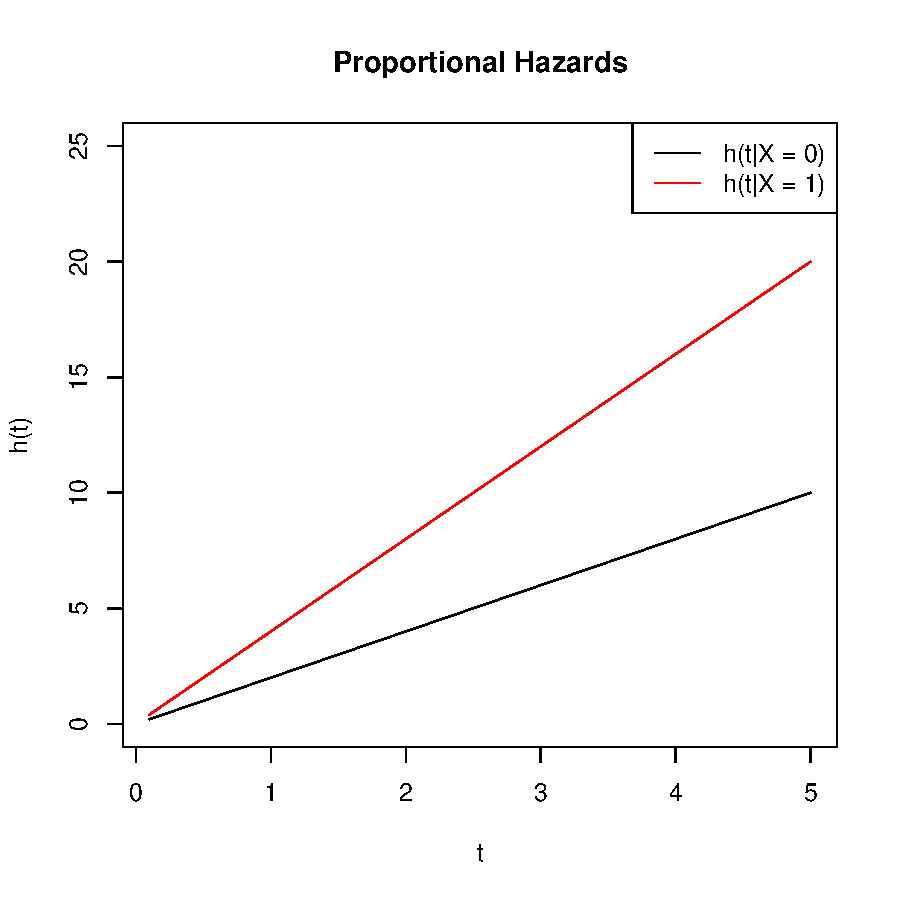
\includegraphics[width = 2in, height = 2in]{survival_present-ph.pdf}
#\end{center}
#\pause
#If one unit change in $X$ doubles the hazard rate, then it doubles the
#hazard rate at all $t$.
#\end{frame}
